\documentclass{beamer}
\usepackage{media9}


%Graphics and Videos
\usepackage{graphicx} %The mode "LaTeX => PDF" allows the following formats: .jpg  .png  .pdf  .mps
\graphicspath{{./images/}} %Where the figures folder is located
\usepackage{media9}
\addmediapath{./videos/}


\usetheme{Boadilla}
\title{Cavity QED mit Mikrowellen Resonanz}
\subtitle{Nobel Preis (2012) von Serge Haroche}
\author{Angelo Brade}
%\institute{Rhenish Friedrich Wilhelm University of Bonn}
\institute{University of Bonn}
\date{\today}


\makeatother
\setbeamertemplate{footline}
{
  \leavevmode%
  \hbox{%
  \begin{beamercolorbox}[wd=.4\paperwidth,ht=2.25ex,dp=1ex,center]{section in head/foot}%
    \usebeamerfont{section in head/foot}\insertsectionhead
  \end{beamercolorbox}%
  \begin{beamercolorbox}[wd=.2\paperwidth,ht=2.25ex,dp=1ex,center]{author in head/foot}%
    \usebeamerfont{author in head/foot}\insertshortauthor
  \end{beamercolorbox}%
  \begin{beamercolorbox}[wd=.4\paperwidth,ht=2.25ex,dp=1ex,center]{title in head/foot}%
    \usebeamerfont{title in head/foot}\insertshorttitle\hspace*{1em}
    \insertframenumber{} / \inserttotalframenumber\hspace*{1ex}
  \end{beamercolorbox}}%
  \vskip0pt%
}
\makeatletter
\setbeamertemplate{navigation symbols}{}



\begin{document}
\begin{frame}
	\titlepage
\end{frame}
\begin{frame}
	\frametitle{Outline}
	\tableofcontents
\end{frame}

\section{Historische Einordnung}
\subsection{Vorrangegangene Entwicklungen}
\begin{frame}
	\frametitle{Vorrangegangene Entwicklung}
\end{frame}
\subsection{Schrödingers Katze}
\begin{frame}
	\frametitle{Schrödingers Katze}
\end{frame}
\section{Mikrowellen Resonator}
\subsection{Stehende Wellen und Moden}
\begin{frame}
	\begin{enumerate}
		\item Einlaufende Welle
		      \begin{itemize}
			      \item $E_1=A e^{i(\omega t - kx)}$
		      \end{itemize}
		\item Reflexion
		      \begin{itemize}
			      \item Umkerhung der Phase $kx \rightarrow -kx$ und Phasenverschiebung $\pi$
		      \end{itemize}
		\item Auslaufende Welle
		      \begin{itemize}
			      \item $E_1 \rightarrow E_2=A e^{i(\omega t + kx + \pi)}$
		      \end{itemize}
		\item Interferenz nach Superpositionsprinzip
		      \begin{itemize}
			      \item $E_{\text{tot}} = E_1 + E_2 = 2Ae^{i(\omega t+\frac{\pi}{2})}\cos{(kx+\frac{\pi}{2})}$
			      \item $\Rightarrow y(x,t)=\text{Re}(E_{\text{tot}})=2A\sin{(\omega t)}\sin{(kx)}$
		      \end{itemize}
	\end{enumerate}
\end{frame}
\begin{frame}
	\frametitle{Stehende Wellen und Moden}
	\begin{center}
		\includemedia[
			activate=onclick,
			width=0.4\textwidth
		]{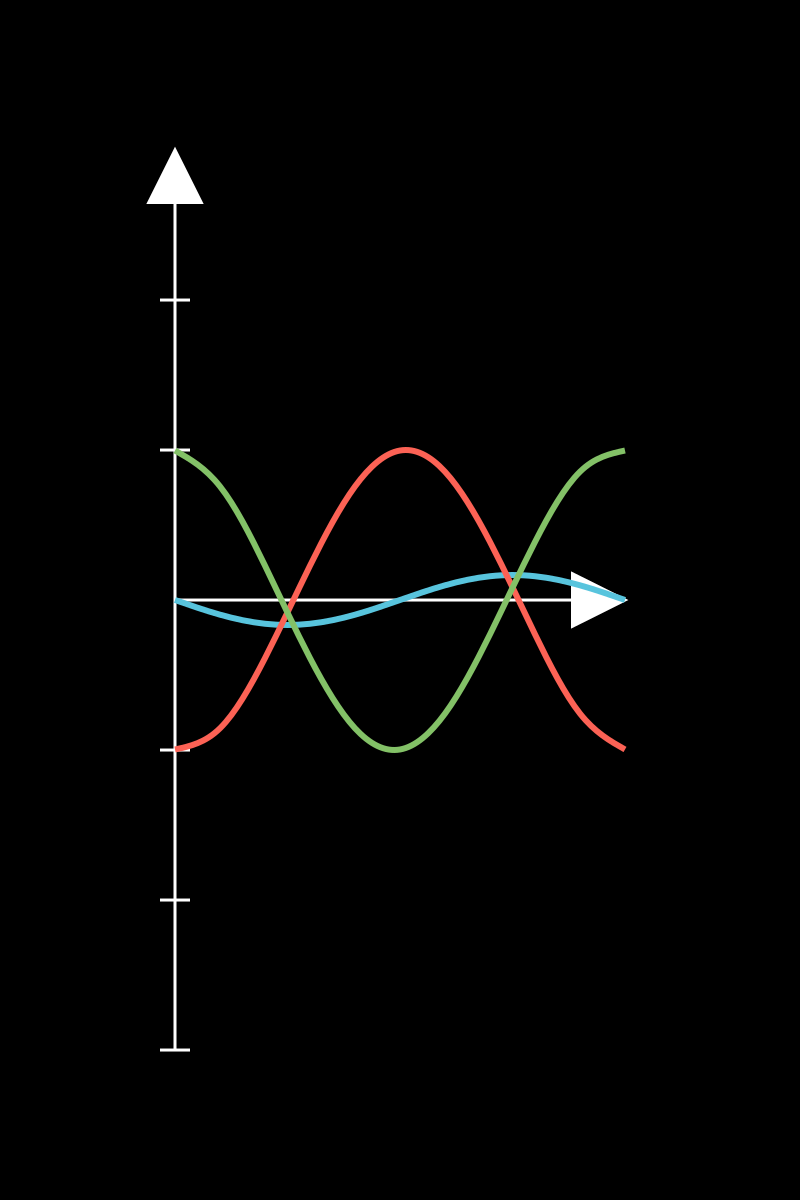
\includegraphics{images/stehwelle.png}}{videos/stehwelle.swf}
	\end{center}
\end{frame}
\begin{frame}
  \includemedia[
  width=0.6\linewidth,
  height=0.45\linewidth,
  activate=onclick,
  addresource=example.mp4,
  flashvars={
     source=example.mp4
    &autoPlay=true
  }
]{\fbox{Click to play}}{videos/stehwelle.swf}
\end{frame}
\subsection{Spiegel}
\begin{frame}
	\frametitle{Spiegel}
	\begin{itemize}
		\item Luft und Spiegel können als Leiter betrachtet werden
		\item Reflektionskoeffizient: $r=\frac{Z_A-Z_W}{Z_A+Z_W}$
		      \begin{itemize}
			      \item $Z_A$:=Abschlusswiderstand
            \item $Z_W$:=Wellenwiderstand
		      \end{itemize}
		\item Für Metalle gilt: $Z_M=\sqrt{\frac{i\omega\mu}{\sigma+i\omega\epsilon}}$ mit $\sigma$:=Leitfähigkeit
		\item Spiegel (Abschluss) aus Metall: $Z_A=Z_M$
		\item $\Rightarrow \lim_{\sigma\rightarrow\infty}r=-1$
		\item $\Rightarrow$ \textbf{Leitfahigkeit soll maximiert werden}
	\end{itemize}
\end{frame}
\subsection{Q Faktor}
\begin{frame}
	\frametitle{Q Faktor}
	\begin{itemize}
		\item $Q:=\frac{\text{gespeicherte Energie}}{\text{Energieverlust}}$
		\item $r\rightarrow \pm1\Leftrightarrow Q\rightarrow\infty$
		\item Spiegel von Haroche: $Q \approx 10^6 \hat{=} \tau_{\text{ph.}}=1$ms
		      \begin{itemize}
            \item \textbf{Zu niedrig}
		      \end{itemize}
	\end{itemize}
\end{frame}
\begin{frame}
	\Large\center Wie kann man die Leitfähigkeit erhöhen?
\end{frame}
\begin{frame}
	\begin{itemize}
		\frametitle{Q Faktor}
		\item Spiegel von Meschede: $Q \approx 10^{10} \hat{=} \tau_{\text{ph.}}=10$s
		      \begin{itemize}
			      \item nutzt Supraleiter $\Leftrightarrow Z_M \approx 0 \Leftrightarrow r\approx-1$\
		      \end{itemize}
    \item Haroche nutzt Spiegel von Meschede
    \item Meschede wird Postdoc von Haroche
	\end{itemize}
\end{frame}
\section{QND}
\begin{frame}
	\frametitle{Vorrangegangene Entwicklung}
\end{frame}
\subsection{Rydberg-Atom}
\begin{frame}
	\frametitle{Rydberg-Atom}
\end{frame}
\subsection{Ramsey Interferometer}
\begin{frame}
	\frametitle{Ramsey Interferometer}
\end{frame}
\section{Schrödingers Kätzchen}
\begin{frame}
	\frametitle{Schrödingers Kätzchen}
\end{frame}
\section{Zusammenfassung}
\begin{frame}
	\frametitle{Zusammenfassung}
\end{frame}
\begin{frame}
	\frametitle{Title}
	Geschichte
\end{frame}
\end{document}
